% =====================================================================
%  Component showcase for dbfdoc.cls: every building block on real-looking
%  pages. ALL VALUES ARE ILLUSTRATIVE, NOT ANALYSIS.
%  Build:  ../tools/build.sh showcase.tex     (run make_figures.py first)
% =====================================================================
\def\dbfroot{..}
\documentclass{dbfdoc}
\dbfsetdoc{Towed-Sensor Surveillance UAV}{Proposal}{AUM-DBF-27-SHOWCASE}{A}
\dbfsetdate{30 Oct 2026}

\begin{document}

\begin{frontmatter}
\section{Executive Summary}
\noindent\begin{minipage}[t]{0.605\textwidth}
\setlength\parindent{1.15em}\noindent
The \dbfuniversity{} proposes a 6-ft-span, electrically powered surveillance UAV that ships sensor containers in Mission~2, deploys and recovers a light-commanded towed sensor in Mission~3, and protects that sensor through repeated drops in the Ground Mission. The objective is to maximize competition score by completing every mission on the first attempt, then pushing the variables that move the score most.

A coupled scoring model shows that mission completion alone is worth 4.5 of the 7.5 available mission points, and that sensor weight is the only design variable present in three of the four mission scores. The design is therefore built around a dense, finned sensor and a powered deployment-and-recovery reel engineered for first-attempt reliability. Weighted trade studies select a high-wing, single-tractor monoplane with tricycle gear and a ventral sensor bay. Preliminary sizing yields the targets at right and a predicted total mission score of 6.12. A six-function team executes a three-prototype build-and-test campaign that flies the competition aircraft by 1~March~2027.
\end{minipage}\hfill
\begin{minipage}[t]{0.365\textwidth}
\vspace{-11pt}
\begin{dbfpanel}[Design at a Glance / Illustrative values]
\dbfplaceholder{\linewidth}{1.05in}{Concept render}\par\vspace{6pt}
\dbfreadout{Wingspan}{5.95}{ft}\hfill\dbfreadout{M2 gross weight}{14.80}{lb}\dbfreadoutgap
\dbfreadout{Sensor weight}{2.20}{lb}\hfill\dbfreadout{M2 payload}{6}{units}\dbfreadoutgap
\dbfreadout{M2 five-lap time}{171.40}{s}\hfill\dbfreadout{M3 laps}{7}{laps}\dbfreadoutgap
\dbfreadout{GM drop height}{60}{in}\hfill\dbfreadout{Pred. mission score}{6.12}{/ 7.50}
\end{dbfpanel}
\end{minipage}
\end{frontmatter}

\section{Management Summary}
\subsection{Team Organization}
The team is organized by function rather than by aircraft component, so that every scored subsystem has a single accountable owner. A Team Lead manages schedule, budget and the faculty interface; a Chief Engineer owns configuration control and integration. Six sub-teams report to them (Table~\ref{tab:roles}). Sensor Systems is new this year and owns the sensor, the deployment-and-recovery (D\&R) mechanism, the shipping container and its rigging, which together touch three of the four mission scores.

\begin{table}[t]
\caption{Sub-team responsibilities and required skill sets.}\label{tab:roles}
\begin{dbftable}{colspec={X[1.05,l] X[1.6,l] X[1.25,l]}}
Sub-team & Responsibility & Key skills \\
Aero \& Perf. & Sizing, lap model, stability & XFLR5, AVL, Python \\
Structures & Airframe design, load tests & CAD, FEA, composites \\
Propulsion & Motor, prop, battery, ESC & eCalc, thrust stand \\
Sensor Systems & Sensor, D\&R reel, container & Embedded C, mechanisms \\
Flight Ops & Pilot, ground crew, checklists & AMA pilot, RC setup \\
Business & Budget, travel, documents & Finance, LaTeX \\
\end{dbftable}
\end{table}

Sub-team leads meet weekly with the Chief Engineer; design decisions are frozen at two internal reviews (PDR and CDR) before material is cut. Each lead maintains a requirements tracker keyed to the requirement IDs defined in Section~3.1, so a judge, a mentor or a new member can trace any part of the aircraft back to the rule that drove it.

\subsection{Schedule and Milestones}
The schedule (Fig.~\ref{fig:gantt}) is built backward from the fly-off and holds three flying prototypes: a proof-of-concept airframe, a sensor-system test bed, and the competition aircraft. Every milestone carries an owner and a pass criterion rather than a date alone.

\begin{figure*}[t]
\dbfplaceholder{\textwidth}{1.55in}{Gantt chart / full width / 5 swim lanes}
\caption{Program schedule. Two internal design reviews gate manufacturing; the sensor system flies on a test bed six weeks before the competition aircraft.}\label{fig:gantt}
\end{figure*}

\subsection{Budget}
Table~\ref{tab:budget} lists all program costs, including travel from Kuwait to Tucson, test articles and a 12\% contingency. Funding is drawn from the engineering college allocation and two industry sponsors.

\begin{table}[t]
\caption{Program budget (illustrative values).}\label{tab:budget}
\begin{dbftable}{colspec={X[l] Q[r] Q[r]}, row{Z}={font=\dbftotalrow}, hline{Y}={0.4pt,dbfGraphite}}
Category & Cost (USD) & Share \\
Airframe materials & 2,150 & 7\% \\
Propulsion and avionics & 1,980 & 6\% \\
Sensor system and test articles & 1,240 & 4\% \\
Tooling and consumables & 860 & 3\% \\
Travel and lodging & 20,400 & 66\% \\
Fees and memberships & 950 & 3\% \\
Contingency (12\%) & 3,310 & 11\% \\
Total & 30,890 & 100\% \\
\end{dbftable}
\end{table}

\section{Conceptual Design Approach}
\subsection{Scoring Model and Sensitivity Study}
The total mission score is the sum of four mission scores, each a fixed completion credit plus a term normalized by the best team in the field:
\begin{equation}
\begin{aligned}
S_\mathrm{M} &= M_1 + \Bigl[1 + \tfrac{(W/t)}{(W/t)_\mathrm{max}}\Bigr]
  + \Bigl[2 + \tfrac{N W_s}{(N W_s)_\mathrm{max}}\Bigr] \\
 &\quad + \Bigl[0.5 + \tfrac{W_s h}{(W_s h)_\mathrm{max}}\Bigr]
\end{aligned}
\end{equation}
where $W$ is the Mission~2 payload weight, $t$ the five-lap time, $N$ the Mission~3 lap count, $W_s$ the sensor weight and $h$ the declared drop height.\footnote{AIAA, \emph{2026--27 Design, Build, Fly Rules}, Draft, Sep.~2026, Sec.~3.3.}
Completion credits total 4.5 points, so an aircraft that finishes every mission already holds 60\% of the available mission score. Only 17 of 89 teams completed all missions in 2026,\footnote{AIAA, \emph{2026 Design, Build, Fly Competition Summary}, Apr.~2026.} which makes first-attempt reliability the first design driver.

\begin{figure}[t]
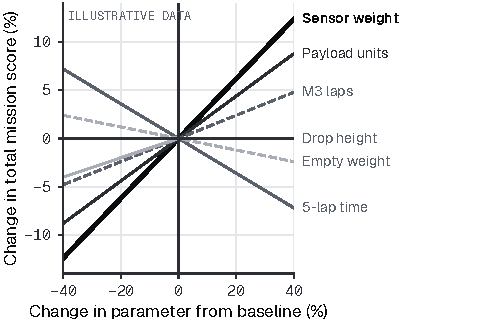
\includegraphics[width=\columnwidth]{figures/sensitivity.pdf}
\caption{Sensor weight moves the total mission score more than any other parameter, because it appears in the M2, M3 and GM terms.}\label{fig:sens}
\end{figure}

Figure~\ref{fig:sens} perturbs each design variable about the baseline while holding the others fixed. Sensor weight dominates, followed by Mission~2 payload units; drop height saturates at the 60-in cap, so a heavier sensor, not a higher drop, is the route to a higher Ground Mission score.

\subsection{Configuration Trade Studies}
Figure-of-merit weights are taken directly from the sensitivity results, so the configuration is selected for the score it can earn rather than by convention (Table~\ref{tab:trade}).

\begin{table}[t]
\caption{Configuration trade (scores 1--5; selected option inverted).}\label{tab:trade}
\begin{dbftable}{colspec={X[l] Q[c] Q[c] Q[c] Q[c]}, column{4}={bg=dbfAccentTint}, cell{1}{4}={bg=dbfInk, fg=white}, row{Z}={font=\dbftotalrow}, hline{Y}={0.4pt,dbfGraphite}}
Criterion (wing position) & Wt. & Low & High & Mid \\
Sensor bay access & 0.30 & 3 & 5 & 2 \\
Tow-line clearance & 0.25 & 2 & 5 & 3 \\
Structural weight & 0.20 & 4 & 4 & 3 \\
Roll stability & 0.15 & 3 & 5 & 4 \\
Manufacturability & 0.10 & 4 & 4 & 2 \\
Weighted total & 1.00 & 3.05 & \dbfselected{4.70} & 2.75 \\
\end{dbftable}
\end{table}

A high wing clears the ventral sensor bay and keeps the tow line well below the empennage during deployment and recovery, the two phases in which a towed body is most likely to strike the aircraft.

\subsection{Preliminary Design and Sizing}
\subsubsection{Sizing method}
Wing and power loading are selected on a constraint diagram (Fig.~\ref{fig:constraint}) built from the turn, climb, cruise and stall requirements at Tucson density altitude.\footnote{Raymer, D.~P., \emph{Aircraft Design: A Conceptual Approach}, 6th ed., AIAA, Reston, VA, 2018.}

\begin{figure}[t]
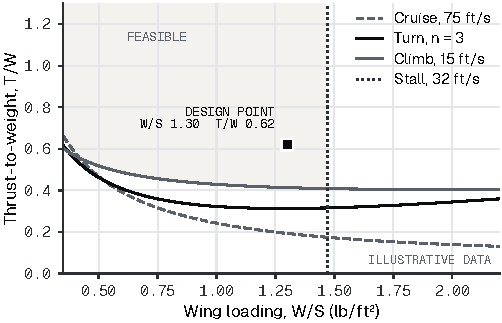
\includegraphics[width=\columnwidth]{figures/constraint.pdf}
\caption{The sustained 3-g turn sets the power requirement; the design point holds an 0.21 margin in T/W for gusts and towed-sensor drag.}\label{fig:constraint}
\end{figure}

\subsubsection{Aircraft parameters}
Table~\ref{tab:params} summarizes the preliminary design. All weights are Mission~2 values unless noted.

\begin{table}[t]
\caption{Preliminary design parameters (illustrative values).}\label{tab:params}
\begin{dbftable}{colspec={X[l] Q[r] Q[l]}}
Parameter & Value & Unit \\
Wingspan & 5.95 & ft \\
Wing area & 6.10 & ft² \\
Aspect ratio & 5.80 & -- \\
Gross weight, M2 & 14.80 & lb \\
Battery energy & 99.90 & Wh \\
Cruise speed & 75.00 & ft/s \\
\end{dbftable}
\end{table}

\subsubsection{Sensor and D\&R system}
The sensor is a finned, 9-in body carrying its own battery, light controller and three LED groups; ballast sits in an internal bay so its weight can be trimmed without changing its shape. A powered reel pays out the tow line to 1.5 times the span and recovers it on command. The command signal reaches the sensor through the tow line itself, which makes the electrical path through the rotating reel (a slip ring) the critical technology (Fig.~\ref{fig:block}). The aircraft is flown pilot-in-the-loop at all times: no autopilot or flight controller is carried, and stabilization is limited to optional rate gyros.

\begin{figure}[t]
\dbfplaceholder{\columnwidth}{1.45in}{Signal block diagram}
\caption{Command path from the receiver through the reel slip ring to the sensor light controller.}\label{fig:block}
\end{figure}

\subsection{Mission Design Approach and Scoring Targets}
Each mission target in Table~\ref{tab:targets} comes from the lap and energy model rather than from experience, so every number can be traced to a requirement and a test.

\begin{table}[t]
\caption{Mission targets and predicted scores (illustrative values).}\label{tab:targets}
\begin{dbftable}{colspec={Q[l] X[l] Q[r]}, row{Z}={font=\dbftotalrow}, hline{Y}={0.4pt,dbfGraphite}}
Mission & Target & Score \\
M1 Staging & Waived; credited by M2 & 1.00 \\
M2 Delivery & 6 units, 13.20 lb, 171.40 s & 1.62 \\
M3 Sensor & 7 laps at 2.20 lb & 2.55 \\
GM Ground & 60 in at 2.20 lb & 0.95 \\
Total mission score & & 6.12 \\
\end{dbftable}
\end{table}

Mission~1 is waived under the new rule because a successful Mission~2 earns the same credit with one fewer flight, a material saving when the field averaged 2.2 attempts per team in 2026.

\begin{itemize}
\item Square markers in Steel; compact list spacing on the 1.5-line grid.
\item Drafting notes and unfinished values are part of the system:
\end{itemize}
\dbfnote{Drafting notes look like this and vanish with the \texttt{final} class option.}
An unfinished number renders as \dbftbd{M2 time} and is counted by the build script.

\end{document}
